\documentclass[a4paper,10pt]{article}
\usepackage[spanish]{babel}
\usepackage[utf8]{inputenc}
\usepackage{booktabs}
\usepackage{hyperref}
\usepackage{fontawesome}
\usepackage{graphicx}
\usepackage{listings}
\usepackage{color}
\usepackage{fancyvrb}

\definecolor{dkgreen}{rgb}{0,0.6,0}
\definecolor{gray}{rgb}{0.5,0.5,0.5}
\definecolor{mauve}{rgb}{0.58,0,0.82}

\lstset{frame=tb,
  language=C,
  aboveskip=3mm,
  belowskip=3mm,
  showstringspaces=false,
  columns=flexible,
  basicstyle={\small\ttfamily},
  numbers=none,
  numberstyle=\tiny\color{gray},
  keywordstyle=\color{blue},
  commentstyle=\color{dkgreen},
  stringstyle=\color{mauve},
  breaklines=true,
  breakatwhitespace=true,
  tabsize=3
}

\lstset{}

\title{
    
\includegraphics[width=5cm]{plots/fiuba.png}\\
    Programación MIPS\\
    Trabajo Práctico 1\\}
\date{}
\author{}

\begin{document}

    \pagenumbering{gobble}
    \maketitle
    \begin{table}[h!]
      \centering
      \begin{tabular}{ccc}
        \toprule
        Apellido y Nombre & Padrón & Correo electrónico \\
        \midrule
        Blanco, Sebastian & 98539 & sebastian.e.blanco@gmail.com\\
        Lavandeira, Lucas & 98042 & lucaslavandeira@gmail.com\\
        Llauró, Manuel Luis & 95736 & llauromanuel@gmail.com\\
        \bottomrule
      \end{tabular}
    \end{table}

    \texttt{GitHub} \faGithub:
    \url{https://github.com/lucaslavandeira/palindrome-MIPS}
      
\newpage
    \pagenumbering{arabic}
    \tableofcontents

\newpage

    \section{Introducción}
El objetivo de este trabajo práctico familiarizarse con las herramientas de software, implementando un programa para procesar archivos
de texto por línea de comando en MIPS: el programa recibirá los archivos o streams de
entrada y salida, y deberá imprimir aquellas palabras del archivo de entrada
(componentes léxicos) que sean palíndromos.

    \section{Diseño e implementación}
    El programa se divide en 2 partes, el arranque y configuración por un lado, y por el otro el procesamiento.
    \\
    La sección de arranque y configuración consiste en el procesamiento de las lineas de comandos, y la apertura y cierre de archivos. Esta parte del programa esta escrita en C, y para el procesamiento hace un llamado a la función \texttt{palindrome(fdIn, ibytes, fdOut, obytes)}.
    \\
    Y la sección de Procesamiento es en definitiva la escritura de la función palindrome, escrita en MIPS32, junto a las distintas funciones llamadas por palindrome, creadas para resolver la consigna del trabajo practico.
    
    Para la función palindrome se decidió crear un stack de 80 bytes. 
    Las funciónes que se crearon para completar el procesamiento son \texttt{int putch(fd, buffer, oBytes, pos,  c)}  y \texttt{int getch(fd, buffer,  iBytes,  pos)} para cumplir por lo pedido con la consigna de leer y escribir en el archivo usando las Syscall lo menos posible. Esto se resuelve creando buffers que van almacenando de partes lo que se lee y otro buffer que almacena lo que se va escribiendo. De esta manera solo al llenarse el buffer de escritura o vaciarse de lectura, se usan las Syscalls y se lee o se escribe en el archivo respectivamente.
    
    Además de estas funciones, fue necesario crear las funciones \texttt{char mytolower(c)}, la cual devuelve el valor de una en minúscula, y "mymalloc" y "myrealloc" que hace de funciones malloc y realloc de C, pero reprogramadas en MIPS32.
    
    Otras funciones programadas fueron \texttt{bool isCapicua(word, len)}, que indica si una palabra es o no capicúa, y por último la función \texttt{bool belongsToSpace( c)} que me indica si el caracter pertenece o no a la definición caracteres que forman palabras, estipulados en el Trabajo práctico anterior. 
    \\
    La combinación de estas funciones logran resolver el objetivo pedido.

    \section{Modo de uso}
El ejecutable compilado no tiene dependencias con otros archivos o librerías, y puede moverse y ejecutarse desde cualquier directorio. Al ejecutarse desde una terminal sin argumentos adicionales, leerá de la entrada estándar palabras (es decir, componentes léxicos con caracteres alfanuméricos, y dígitos del 0 al 9), e imprimirá por la salida estándar aquellos que sean palíndromos. Al leer un carácter del final de archivo (\texttt{EOF}), finalizará su ejecución.
El programa, adicionalmente, acepta varios parámetros adicionales (todos opcionales):
\begin{itemize}
    \item \texttt{-h}: Muestra en pantalla los parámetros aceptados y finaliza su ejecución
    \item \texttt{-V}: Muestra la versión del programa compilado y finaliza su ejecución
    \item \texttt{-i <archivo>}: Lee la entrada del programa desde el archivo especificado
    \item \texttt{-o <archivo>}: Imprime la salida del programa al archivo especificado
    \item \texttt{-I, o --ibuf-bytes <valor numérico>}: determina el tamaño en bytes del buffer de entrada. El valor por defecto a usar es 1.
    \item \texttt{-O, o --obuf-bytes <valor numérico>}: nos permite dimensionar el buffer se salida. El valor por defecto también es 1.
\end{itemize}
El programa tiene dos códigos de salida: 0 en funcionamiento correcto, y 1 en caso de error, causado por la lectura inválida de un archivo de entrada, o escritura inválida del archivo de salida.
    \section{Herramientas utilizadas y testing}
El funcionamiento correcto del proyecto se sometió a prueba haciendo uso de varias herramientas propias de los entornos Unix-like, principalmente de \textit{bash}, y de las \textit{coreutils} de GNU, para armar un simple script que busque archivos de entrada en un directorio, y compare los resultados (tanto la escritura de un archivo del parámetro \texttt{-o} como de la salida estándar) con archivos de salida. Para facilitar la compilación del programa (y del informe) se utilizó un simple Makefile. También se usa como compilador el designado por la cátedra, \texttt{gcc}.
\newpage
    \section{Performance según el tamaño del buffer de entrada}
    ibytes, como ya se ha mencionado, es el tamaño del buffer de entrada. Observamos que la velocidad del programa incrementa a medida que la capacidad del buffer aumenta y esto era de esperarse, ya que al aumentar el tamaño del buffer se producen menos lecturas del archivo. Estos resultados se ven reflejados en el siguiente gráfico:\\\\
    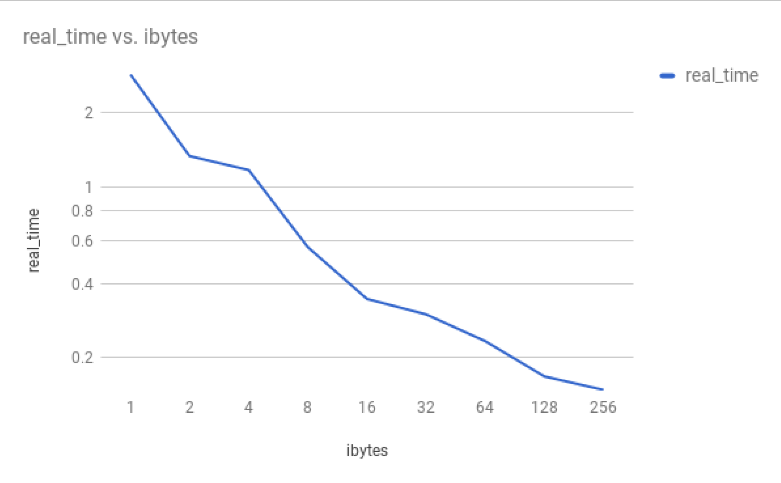
\includegraphics[width=14cm]{plots/times.png}\\
    
    \begin{Verbatim}
    Los tiempos de ejecución del TP0 fueron:
    real    0m0.566s
    user    0m0.386s
    sys     0m0.008s
    \end{Verbatim}
    Donde el real time es el tiempo total de la ejecución del programa. Estos resultados fueron obtenidos de hacer el promedio de varias mediciones.\\
    Observando los datos del TP0 y el gráfico de este mismo Trabajo, es fácil darse cuenta que a medida que el tamaño del buffer se agranda, disminuimos el tiempo de ejecución, superando al del TP0 rápidamente.
    
    \section{Problemas encontrados}
El desarrollo del programa no tuvo mayores inconvenientes, si bien fue difícil acostumbrarse a programar en MIPS, con un poco de practica e investigación de, como por ejemplo la manera de desreferenciar un puntero, se pudo completar el trabajo practico en buenas condiciones.

    \section{Casos de prueba}
Se realizaron para el trabajo práctico 6 casos de pruebas distintos para verificar el correcto funcionamiento del código.\\
Para correr las pruebas se creó un archivo \texttt{run\char`_tests.sh}, el cual corre todas las pruebas del directorio "test" (el mismo se lo puede encontrar el git, o en el pendrive del tp).\\
A continuación se presentan las pruebas realizadas:\\

Prueba: "\texttt{help.in}" \\
    Argumentos de entrada: -h\\
    La salida esperada en "help.out": (vacío)\\
    La salida esperada en "help.stdout":
        \begin{Verbatim}
Usage:
  tp1 -h
  tp1 -V
  tp1 [options]
Options:
  -V, --version	Print version and quit.
  -h, --help	Print this information.
  -i, --input	Location of the input file.
  -o, --output	Location of the output file.
  -I, --ibuf-bytes	byte-count of the input buffer
  -O, --obuf-bytes	byte-count of the output buffer
Examples:
  tp1 -i ~/input -o ~/output

  \end{Verbatim}
      
Prueba: "\texttt{invalid\char`_arg.in}" \\
    Argumentos de entrada: -invalid\\
    La salida esperada en "invalid\char`_arg.out": (vacío)\\
    La salida esperada en "invalid\char`_arg.stdout":
        \begin{Verbatim}
Invalid argument: -invalid
  \end{Verbatim}
  
  Prueba: "\texttt{long\char`_help.in}" \\
    Argumentos de entrada: --help\\
    La salida esperada en "\texttt{long\char`_help.out}": (vacío)\\
    La salida esperada en "\texttt{long\char`_help.stdout}":
        \begin{Verbatim}
Usage:
  tp1 -h
  tp1 -V
  tp1 [options]
Options:
  -V, --version	Print version and quit.
  -h, --help	Print this information.
  -i, --input	Location of the input file.
  -o, --output	Location of the output file.
  -I, --ibuf-bytes	byte-count of the input buffer
  -O, --obuf-bytes	byte-count of the output buffer
Examples:
  tp1 -i ~/input -o ~/output

  \end{Verbatim}
  
    Prueba: "\texttt{long\char`_palindrome.in}" \\
    Argumentos de entrada: \texttt{-i test/long\char`_palindrome.txt -o run.out}\\
    Archivo \texttt{test/long\char`_palindrome.txt}: \\
    \begin{Verbatim}
    aaaaaaaaaaaaaaaaaaaaaaaaaaaaaaaaaaaaaaaaaaaaaaaaaaaaaaaaaaaaaaaaaaaaaaaaaa
    aaaaaaaaaaaaaaaaaaaaaaaaaaaaaaaaaaaaaaaaaaaaaaaaaaaaaaaaaaaaaaaaaaaaaaaaaa
    aaaaaaaaaaaaaaaaaaaaaaaaaaaaaaaaaaaaaaaaaaaaaaaaaaaaaaaaaaaaaaaaaaaaaaaaaa
    aaaaaaaaaaaaaaaaaaaaaaaaaaaaaaaaaaaaaaaaaaaaaaaaaaaaaaaaaaaaaaaaaaaaaaaaaa
    aaaaaaaaaaaaaaaaaaaaaaaaaaaaaaaaaaaaaaaaaaaaaaaaaaaaaaaaaaaaaaaaaaaaaaaaaa
    aaaaaaaaaaaaaaaaaaaaaaaaaaaaaaaaaaaaaaaaaaaaaaaaaaaaaaaaaaaaaaaaaaaaaaaaaa
    aaaaaaaaaaaaaaaaaaaaaaaaaaaaaaaaaaaaaaaaaaaaaaaaaaaaaaaaaaaaaaaaaaaaaaaaaa
    aaaaaaaaaaaaaaaaaaaaaaaaaaaaaaaaaaaaaaaaaaaaaaaaaaaaaaaaaaaaaaaaaaaaaaaaaa
    aaaaaaaaaaaaaaaaaaaaaaaaaaaaaaaaaaaaaaaaaaaaaaaaaaaaaaaaaaaaaaaaaaaaaaaaaa
    aaaaaaaaaaaaaaaaaaaaaaaaaaaaaaaaaaaaaaaaaaaaaaaaaaaaaaaaaaaaaaaaaaaaaaaaaa
    aaaaaaaaaaaaaaaaaaaaaaaaaaaaaaaaaaaaaaaaaaaaaaaaaaaaaaaaaaaaaaaaaaaaaaaaaa
    aaaaaaaaaaaaaaaaaaaaaaaaaaaaaaaaaaaaaaaaaaaaaaaaaaaaaaaaaaaaaaaaaaaaaaaaaa
    aaaaaaaaaaaaaaaaaaaaaaaaaaaaaaaaaaaaaaaaaaaaaaaaaaaaaaaaaaaaaaaaaaaaaaaaaa
    aaaaaaaaaaaaaaaaaaaaaaaaaaaaaaaaaaaaaa
    \end{Verbatim}
    La salida esperada en "\texttt{long\char`_palindrome.out}": El mismo archivo\\
    La salida esperada en "\texttt{long\char`_palindrome.stdout}": (vacío)\\
  
      Prueba: "\texttt{long\char`_params.in}" \\
    Argumentos de entrada: \texttt{--input test/single\char`_character.txt --output run.out}\\
    Archivo \texttt{test/single\char`_character.txt}: \\
    \begin{Verbatim}
    A
    \end{Verbatim}
    La salida esperada en "\texttt{long\char`_palindrome.out}": A\\
    La salida esperada en "\texttt{long\char`_palindrome.stdout}": (vacío)\\
  
        Prueba: "\texttt{long\char`_version.in}" \\
    Argumentos de entrada: \texttt{--version}\\
    Archivo \texttt{test/single\char`_character.txt}: \\

    La salida esperada en "\texttt{long\char`_palindrome.out}": (vacío)\\
    La salida esperada en "\texttt{long\char`_palindrome.stdout}": \\
    \begin{Verbatim}
    tp0: version 0.2
    \end{Verbatim}
  
    Prueba: "\texttt{multiple\char`_palindrome.in}" \\
    Argumentos de entrada: \texttt{-i test/multiple\char`_palindrome.txt -o run.out}\\
    Archivo \texttt{test/multiple\char`_palindrome.txt}: \\
    \begin{Verbatim}
    Somos los primeros en completar el TP 0.
    Ojo que La fecha de entrega del TP0 es el martes 12 de septiembre.
    \end{Verbatim}
    La salida esperada en "\texttt{multiple\char`_palindrome.out}":\\
        \begin{Verbatim}
    Somos
    0
    Ojo
    \end{Verbatim}
    La salida esperada en "\texttt{multiple\char`_palindrome.stdout}": (vacío)\\
  
    Prueba: "\texttt{no\char`_palindrome.in}" \\
    Argumentos de entrada: \texttt{-i test/no\char`_palindrome.txt -o run.out}\\
    Archivo \texttt{test/no\char`_palindrome.txt}: \\
    \begin{Verbatim}
    Somos los primeros en completar el TP 0.
    Ojo que La fecha de entrega del TP0 es el martes 12 de septiembre.
    \end{Verbatim}
    La salida esperada en "\texttt{no\char`_palindrome.out}":\\
        \begin{Verbatim}
    Somos
    0
    Ojo
    \end{Verbatim}
    La salida esperada en "\texttt{no\char`_palindrome.stdout}": (vacío)\\
    
    
    Prueba: "\texttt{single\char`_character.in}" \\
    Argumentos de entrada: \texttt{-i test/single\char`_character.txt -o run.out}\\
    Archivo \texttt{test/single\char`_character.txt}: \\
    \begin{Verbatim}
    A
    \end{Verbatim}
    La salida esperada en "\texttt{single\char`_character.out}":\\
        \begin{Verbatim}
    A
    \end{Verbatim}
    La salida esperada en "\texttt{single\char`_character.stdout}": (vacío)\\
    
    
    Prueba: "\texttt{underscores.in}" \\
    Argumentos de entrada: \texttt{-i test/underscores.txt -o run.out}\\
    Archivo \texttt{test/underscores.txt}: \\
    \begin{Verbatim}
    _a_ -a- a-b_c_b-a
    \end{Verbatim}
    La salida esperada en "\texttt{underscores.out}":\\
        \begin{Verbatim}
    _a_
    -a-
    a-b_c_b-a
    \end{Verbatim}
    La salida esperada en "\texttt{underscores.stdout}": (vacío)\\
    
        Prueba: "\texttt{numeric.in}" \\
    Argumentos de entrada: \texttt{-i test/numeric.txt -o run.out}\\
    Archivo \texttt{test/numeric.txt}: \\
    \begin{Verbatim}
    1
    9009
    12
    000000000000
    \end{Verbatim}
    La salida esperada en "\texttt{numeric.out}":\\
        \begin{Verbatim}
    1
    9009
    000000000000
    \end{Verbatim}
    La salida esperada en "\texttt{numeric.stdout}": (vacío)\\
    
        Prueba: "\texttt{use\char`_stdout.in}" \\
    Argumentos de entrada: \texttt{-i test/multiple\char`_palindrome.txt -o run.out}\\
    Archivo \texttt{test/multiple\char`_palindrome.txt}: \\
    \begin{Verbatim}
    Somos los primeros en completar el TP 0.
    Ojo que La fecha de entrega del TP0 es el martes 12 de septiembre.
    \end{Verbatim}
    La salida esperada en "\texttt{numeric.out}": (vacío)\\

    La salida esperada en "\texttt{numeric.stdout}": \\
            \begin{Verbatim}
    Somos
    0
    Ojo
    \end{Verbatim}
    
       Prueba: "\texttt{version.in}" \\
    Argumentos de entrada: \texttt{-V}\\
    
    La salida esperada en "\texttt{numeric.out}": (vacío)\\

    La salida esperada en "\texttt{numeric.stdout}": \\
    \begin{Verbatim}
    tp0: version 0.2
    \end{Verbatim}
    
    \section{Salida por consola de la ejecución de \texttt{run\char`_tests.sh}}
    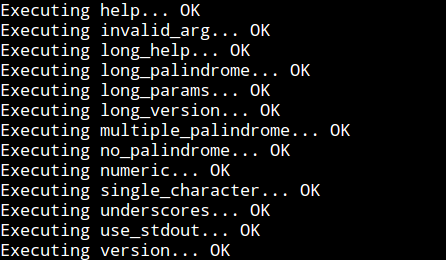
\includegraphics[width=8cm]{plots/runtestout.png}\\
    
    \section{Archivo \texttt{run\char`_tests.sh}}
    \begin{lstlisting}
    #!/bin/bash

TEST_DIR=test/
IN=$TEST_DIR/in/
OUT=$TEST_DIR/out/
ERROR=$TEST_DIR/error/

for case in $(ls $ERROR); do
    rm $ERROR/$case
done

for case in $(ls $IN); do
  ERRORS=false
  if [ -e run.out ]; then 
      rm run.out
  fi
  if [ -e stdout.tmp ]; then
      rm stdout.tmp
  fi
  filename=$(basename ${case%%.*}) 
  printf "Executing $filename... ";
  ./tp0 $(cat $IN/$case) >> stdout.tmp 
  if [ -e run.out ]; then
    diff run.out $OUT/$filename.out >> tmp;
    if [ $? -ne 0 ]; then
      ERRORS=true
    fi
  fi
  diff stdout.tmp $OUT/$filename.stdout >> tmp;
  if [ $? -eq 0 ]; then
    echo "OK"
  else
     ERRORS=true
  fi
  
  if $ERRORS; then
    echo "ERROR"
    cat tmp
    cp stdout.tmp $ERROR/$filename.error.stdout
    if [ -e run.out ]; then
      cp run.out $ERROR/$filename.error
    fi
  fi    
done

if [ -e tmp ]; then
    rm tmp
fi
if [ -e stdout.tmp ]; then
    rm stdout.tmp
fi
    \end{lstlisting}
  
    \newpage
    
    \section{Anexo A: Código C de arranque y configuración}
        \begin{lstlisting}
#define _POSIX_C_SOURCE 1
#include <stdio.h>
#include <string.h>
#include <stdbool.h>
#include <stdlib.h>
//------------------------------------------------------------------------------
// DEFINITIONS
//------------------------------------------------------------------------------
#define ERROR -1
#define SUCCESS 0
#define VERSION "0.1"
const char help_str[] = "Usage:\n"
        "  tp1 -h\n"
        "  tp1 -V\n"
        "  tp1 [options]\n"
        "Options:\n"
        "  -V, --version\tPrint version and quit.\n"
        "  -h, --help\tPrint this information.\n"
        "  -i, --input\tLocation of the input file.\n"
        "  -o, --output\tLocation of the output file.\n"
        "  -I, --ibuf-bytes\tbyte-count of the input buffer\n"
        "  -O, --obuf-bytes\tbyte-count of the output buffer\n"
        "Examples:\n"
        "  tp1 -i ~/input -o ~/output\n";
//------------------------------------------------------------------------------
// EXTERNAL FUNCTIONS
//------------------------------------------------------------------------------
extern int palindrome(int ifd, size_t ibytes, int ofd, size_t obytes);
//------------------------------------------------------------------------------
// EQUAL
//------------------------------------------------------------------------------
bool equal(const char* str1, const char* str2) {
    return strcmp(str1, str2) == 0;
}
//------------------------------------------------------------------------------
// ARG PARSE
//------------------------------------------------------------------------------
int argParse(int argc, char** argv, FILE** descriptors, size_t** ref) {
    int arg = 1;
    const int size = 12;
    const char* flags[] = {"-i", "-o", "-V", "-h", "--version", "--help",
                           "--input", "--output", "-I", "-O", "--ibuf-bytes",
                           "--obuf-bytes"};

    bool std;
    char* flag = "";
    bool isFlagNull;
    while (arg < argc) {
        isFlagNull = true;
        if (argv[arg][0] == '-') {
            for (int i = 0; i < size; i++) {
                if (strcmp(argv[arg], flags[i]) == 0) {
                    flag = argv[arg];
                    isFlagNull = false;
                    break;
                }
            }

            if (equal(flag, "-h") || equal(flag, "--help")) {
                printf("%s\n", help_str);
                *ref[2] = 1;
                return SUCCESS;
            }
            if (equal(flag, "-V") || equal(flag, "--version")) {
                printf("tp1: version %s\n", VERSION);
                *ref[2] = 1;
                return SUCCESS;
            }
            if (isFlagNull) {
                printf("Invalid argument: %s\n", argv[arg]);
                descriptors[0] = NULL;
                return ERROR;
            }
        } else {
            std = equal(argv[arg], "-");
            if ((equal(flag, "-i") || equal(flag, "--input")) && !std) {
                descriptors[0] = fopen(argv[arg], "r");
                if (descriptors[0] == NULL) return ERROR;
            } else if ((equal(flag, "-o") || equal(flag, "--output")) && !std) {
                descriptors[1] = fopen(argv[arg], "w");
                if (descriptors[1] == NULL) return ERROR;
            }
            if ((equal(flag, "-I") || equal(flag, "--ibuf-bytes")) && !std) {
                *ref[0] = (size_t)atoi(argv[arg]);
            }
            if ((equal(flag, "-O") || equal(flag, "--obuf-bytes")) && !std) {
                *ref[1] = (size_t)atoi(argv[arg]);
            }
            flag = "nullStr";
        }
        arg++;
    }
    return SUCCESS;
}
//------------------------------------------------------------------------------
// MAIN
//------------------------------------------------------------------------------
int main(int argc, char** argv) {
    FILE* fdescriptors[2] = {stdin, stdout};
    size_t ibytes = 1, obytes = 1;
    size_t clean_exit = 0;
    size_t* ref[3] = {&ibytes, &obytes, &clean_exit};
    int s = argParse(argc, argv, fdescriptors, ref);
    if (s == ERROR) return 1;
    if (clean_exit) return 0;  // finalizacion limpia, cuando se usa -h o -V

    FILE* archIn = fdescriptors[0];
    FILE* archOut = fdescriptors[1];
    int fdIn = fileno(archIn);
    int fdOut = fileno(archOut);
    if (fdIn == -1 || fdOut == -1) return 1;

    if (palindrome(fdIn, ibytes, fdOut, obytes) == -1) {
        printf("palindrome returned -1\n");
        return 1;
    }
    if (archIn != stdin && fclose(archOut) == EOF) return 1;
    if (archOut != stdout && fclose(archOut) == EOF) return 1;
    return 0;
}
//------------------------------------------------------------------------------
        \end{lstlisting}
        \section{Anexo B: Código Assembly MIPS}
        \subsection{Stack Frames}
        Los Stack frames de las funciones usadas en el programa fueron los siguientes:
        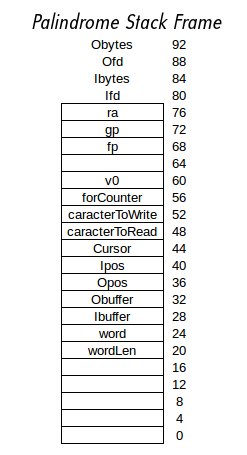
\includegraphics[width=5cm]{plots/PalindromeStack.png}\\
        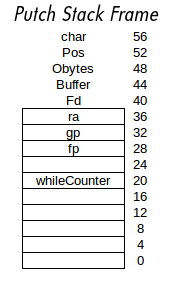
\includegraphics[width=5cm]{plots/putchStack.png}\\
        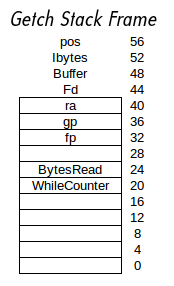
\includegraphics[width=5cm]{plots/getchStack.png}\\
        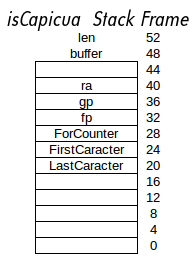
\includegraphics[width=5cm]{plots/isCapicuaStack.png}\\
        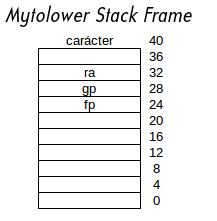
\includegraphics[width=5cm]{plots/mytolowerStack.png}\\
        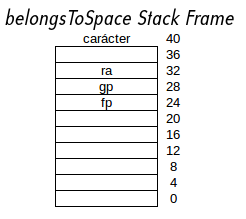
\includegraphics[width=5cm]{plots/belongsToSpaceStack.png}\\
        \subsection{Palindrome.S}
            \begin{lstlisting}
            #include <sys/syscall.h>
#include <mips/regdef.h>
##------------------------------------------------------------------------------
## DEFINITIONS
##------------------------------------------------------------------------------
#ifndef SF_SIZE
#define SF_SIZE 80
#endif

#ifndef RA_POS
#define RA_POS 76
#endif

#ifndef GP_POS
#define GP_POS 72
#endif

#ifndef FP_POS
#define FP_POS 68
#endif

#ifndef RETURN_VALUE_POS
#define RETURN_VALUE_POS 60
#endif

#ifndef FOR_COUNTER_POS
#define FOR_COUNTER_POS 56
#endif

#ifndef CARACTER_TO_WRITE_POS
#define CARACTER_TO_WRITE_POS 52
#endif

#ifndef CARACTER_TO_READ_POS
#define CARACTER_TO_READ_POS 48
#endif

#ifndef CURSOR_POS
#define CURSOR_POS 44
#endif

#ifndef IPOS
#define IPOS 40
#endif

#ifndef OPOS
#define OPOS 36
#endif

#ifndef OBUFFER
#define OBUFFER 32
#endif

#ifndef IBUFFER
#define IBUFFER 28
#endif

#ifndef WORD
#define WORD 24
#endif

#ifndef WORD_LEN_POS
#define WORD_LEN_POS 20
#endif

#ifndef IFD_POS
#define IFD_POS 80
#endif

#ifndef IBYTES_POS
#define IBYTES_POS 84
#endif

#ifndef OFD_POS
#define OFD_POS 88
#endif

#ifndef OBYTES_POS
#define OBYTES_POS 92
#endif

#ifndef INITIAL_SIZE
#define INITIAL_SIZE 1024
#endif

#ifndef SIZE_OF_CHAR
#define SIZE_OF_CHAR 1
#endif

#ifndef EOF
#define EOF -1
#endif

#ifndef ENTER
#define ENTER 10
#endif
##------------------------------------------------------------------------------
## CODIGO EQUIVALENTE EN C
##------------------------------------------------------------------------------
##int palindrome(int ifd, size_t ibytes, int ofd, size_t obytes) {
    ##size_t wordLen = 1024;
    ##char* word = (char*) mymalloc(sizeof(char) * wordLen);
    ##if (word == NULL) return ERROR;
    ##char* iBuffer = (char*) mymalloc(sizeof(char) * ibytes);
    ##if (iBuffer == NULL) {
        ##myfree(word);
        ##return ERROR;
    ##}
    ##char* oBuffer = (char*) mymalloc(sizeof(char) * obytes);
    ##if (oBuffer == NULL) {
        ##myfree(word);
        ##myfree(iBuffer);
        ##return ERROR;
    ##}
    ##size_t iPos = 0;
    ##size_t oPos = 0;
    ##size_t cur = 0;
    ##int c = getch(ifd, iBuffer, ibytes, &iPos);
    ##if (c == -2) {
        ##myfree(word);
        ##myfree(iBuffer);
        ##myfree(oBuffer);
        ##return ERROR;
    ##}

    ##while (c != EOF) {
        ##if (belongsToSpace((char) c)) {
            ##if (cur >= wordLen) {
                ##wordLen *= 2;
                ##word = (char*) myrealloc(word, wordLen);
                ##if (word == NULL) {
                    ##myfree(word);
                    ##myfree(iBuffer);
                    ##myfree(oBuffer);
                    ##return ERROR;
                ##}
            ##}
            ##word[cur] = (char) c;
            ##cur++;
        ##} else {
            ##if (isCapicua(word, cur)) {
                ##for (int i = 0; i < cur; i++) {
                    ##if (putch(ofd, oBuffer, obytes, &oPos, word[i]) == -1) {
                        ##myfree(word);
                        ##myfree(iBuffer);
                        ##myfree(oBuffer);
                        ##return ERROR;
                    ##}
                ##}
            ##}
            ##cur = 0;
        ##}
        ##c = getch(ifd, iBuffer, ibytes, &iPos);
        ##if (c == -2) {
            ##myfree(word);
            ##myfree(iBuffer);
            ##myfree(oBuffer);
            ##return ERROR;
        ##}
    ##}
    ##myfree(word);
    ##myfree(iBuffer);
    ##myfree(oBuffer);
    ##return SUCCESS;
##------------------------------------------------------------------------------
## MACROS
##------------------------------------------------------------------------------
.MACRO callGetch
    lw a0, IFD_POS($fp)  ## guardo en a0 el file descriptor de entrada
    lw a1, IBUFFER($fp)  ## guardo en a1 el buffer de entrada
    lw a2, IBYTES_POS($fp)  ## guardo en a2 el tamaño del buffer de entrada
    addu a3, $fp, IPOS  ## a3 = &pos
    la t9, getch
    jal ra, t9
    li t0, -2  ## t0 = -2
    beq v0, t0, returnError  ## if (c == -2) return ERROR
    sw v0, CARACTER_TO_READ_POS($fp)  ## guardo el caracter leido
.ENDM
.MACRO callPutch
    lw a0, OFD_POS($fp)  ## guardo en a0 el file descriptor de entrada
    lw a1, OBUFFER($fp)  ## guardo en a1 el buffer de entrada
    lw a2, OBYTES_POS($fp)  ## guardo en a2 el tamaño del buffer de entrada
    addu a3, $fp, OPOS  ## a3 = &pos
    lw t0, CARACTER_TO_WRITE_POS($fp)
    sb t0, 16($fp)  ## cargo la posicion de memoria
    la t9, putch
    jal ra, t9
    li t0, -1  ## t0 = -1
    beq v0, t0, returnError  ## if (s == -1) return ERROR
.ENDM
##------------------------------------------------------------------------------
## CODIGO EN MIPS
##------------------------------------------------------------------------------
    .text
    .abicalls
    .align 2
    .globl palindrome
    .ent palindrome
palindrome:
    ##--------------------------------------------------------------------------
    ## Inicializacion del stack frame
    ##--------------------------------------------------------------------------
    .frame $fp, SF_SIZE, ra
    .set noreorder
    .cpload t9
    .set reorder
    subu sp, sp, SF_SIZE
    .cprestore GP_POS
    sw $fp, FP_POS(sp)
    sw ra, RA_POS(sp)
    move $fp, sp
    sw a0, IFD_POS($fp)  # file descriptor
    sw a1, IBYTES_POS($fp)  # buffer
    sw a2, OFD_POS($fp)  # position actual de escritura del buffer
    sw a3, OBYTES_POS($fp)  # capacidad maxima del buffer
    ##--------------------------------------------------------------------------
    ## FIN Inicializacion del stack frame
    ##--------------------------------------------------------------------------

    li t0, INITIAL_SIZE  ##size_t wordLen = 1024;
    sw t0, WORD_LEN_POS($fp)  ## guardo wordLen en el stackFrame

    ## char* word = (char*) malloc(wordLen);
    lw a0, WORD_LEN_POS($fp)  ## cargo a0 con el parametro de la funcion malloc
    la t9, mymalloc  ## cargo en t9 la direccion de la funcion mymalloc
    jal ra, t9
    ## Verifico el error
    li t0, -1
    beq v0, t0, returnWord
    sw v0, WORD($fp)  ## guardo el buffer en el stackFrame

    ## char* iBuffer = (char*) malloc(iBytes);
    lw a0, IBYTES_POS($fp)  ## cargo a0 con el parametro de la funcion malloc
    la t9, mymalloc  ## cargo en t9 la direccion de la funcion mymalloc
    jal ra, t9
    ## Verifico el error
    li t0, -1
    beq v0, t0, returnIBuffer
    sw v0, IBUFFER($fp)  ## guardo el buffer en el stackFrame

    ## char* oBuffer = (char*) malloc(oBytes);
    lw a0, OBYTES_POS($fp)  ## cargo a0 con el parametro de la funcion malloc
    la t9, mymalloc  ## cargo en t9 la direccion de la funcion mymalloc
    jal ra, t9
    ## Verifico el error
    li t0, -1
    beq v0, t0, returnOBuffer
    sw v0, OBUFFER($fp)  ## guardo el buffer en el stackFrame

    sw zero, IPOS($fp)  ## IPos = 0
    sw zero, OPOS($fp)  ## OPos = 0
    sw zero, CURSOR_POS($fp)  ## size_t cur = 0;
    callGetch
while:
    ## while (c != EOF)
    li t0, EOF
    lw t1, CARACTER_TO_READ_POS($fp)  ## t1 = c
    beq t1, t0, returnSuccess  ## if (c == EOF) sale del while
    ##--------------------------------------------------------------------------
    ## if (belongsToSpace(c))
    ##--------------------------------------------------------------------------
    ## bool belongs = belongsToSpace(c);
    lw a0, CARACTER_TO_READ_POS($fp)  ## t1 = c
    la t9, belongsToSpace
    jal ra, t9
    ## true = 1; false = 0
    li t0, 0  ## t0 = false
    beq v0, t0, else  ## if (belongsToSpace(c) == false) sale del if
    ##--------------------------------------------------------------------------
    ## if (cur >= wordLen)
    ##--------------------------------------------------------------------------
    lw t0, CURSOR_POS($fp)  ## t0 = cur
    lw t1, WORD_LEN_POS($fp)  ## t1 = wordLen
    subu t0, t0, t1  ## t0 = cur - wordLen
    bltz t0, beforeElse   ## if (cur - wordLen < 0) sale del if
    ##--------------------------------------------------------------------------
    ##wordLen *= 2;
    lw t1, WORD_LEN_POS($fp)  ## t1 = wordLen
    sll t1, t1, 1  ## t1 = wordLen*2
    sw t1, WORD_LEN_POS($fp)  ## wordLen *= 2
    ##word = (char*) realloc(word, wordLen);
    lw a0, WORD($fp)
    lw a1, WORD_LEN_POS($fp)
    la t9, myrealloc
    jal ra, t9
    ## Verificar el error, es decir, if (word == NULL) return ERROR;
    li t0, -1
    beq v0, t0, returnError
    sw v0, WORD($fp);

beforeElse:
    ## word[cur] = c;
    lw t1, CURSOR_POS($fp)  ## t1 = cur
    lw t0, WORD($fp)
    addu t0, t0, t1  ## t0 = word + cur
    lw t1, CARACTER_TO_READ_POS($fp)  ## t1 = c
    sb t1, 0(t0)  ##  *(word+cur) = c

    ## cur++;
    lw t1, CURSOR_POS($fp)  ## t1 = cur
    addu t1, t1, 1   ## t1++
    sw t1, CURSOR_POS($fp)  ## c++
    j endWhile

else:
    ##--------------------------------------------------------------------------
    ##if (isCapicua(word, cur))
    ##--------------------------------------------------------------------------
    lw a0, WORD($fp)
    lw a1, CURSOR_POS($fp)
    la t9, isCapicua
    jal ra, t9
    ## true = 1; false = 0
    li t0, 0  ## t0 = false
    beq v0, t0, afterIf  ## if (isCapicua(word, cur) == false) saltea el if
    ##for (int i = 0; i < cur; i++)
    sw zero, FOR_COUNTER_POS($fp)  ## i = 0
for:
    lw t0, FOR_COUNTER_POS($fp)  ## t0 = i
    lw t1, CURSOR_POS($fp)  ## t1 = cur
    subu t3, t0, t1  ## t3 = i - cur
    bgez t3, endFor  ## if i >= cur termino el for y salto a afterIf

    lw t3, WORD($fp)  ## t3 = word
    lw t0, FOR_COUNTER_POS($fp)  ## t0 = i
    addu t3, t0, t3  ## t3 = word + i
    lb t3, 0(t3)  ## t3 = *(word + i)
    sb t3, CARACTER_TO_WRITE_POS($fp)
    callPutch
    lw t0, FOR_COUNTER_POS($fp)  ## t0 = i
    addu t0, t0, 1  ## i++
    sw t0, FOR_COUNTER_POS($fp)  ## salvo el contador del for
    j for
endFor:
    la t0, ENTER
    sb t0, CARACTER_TO_WRITE_POS($fp)
    callPutch

afterIf:
    sw zero, CURSOR_POS($fp)  ##cur = 0;

endWhile:
    callGetch
    j while

returnError:
    li t0, -1  ## return -1; Error
    sw t0, RETURN_VALUE_POS($fp)
    j return

returnSuccess:
    lb t0, CARACTER_TO_READ_POS($fp)
    sb t0, CARACTER_TO_WRITE_POS($fp)
    callPutch
    li t0, 0  ## return Success
    sw t0, RETURN_VALUE_POS($fp)
##------------------------------------------------------------------------------
## RETURN
##------------------------------------------------------------------------------
return:
    ## myfree(oBuffer)
    lw a0, OBUFFER($fp)  ## cargo a0 con el parametro de la funcion myfree
    la t9, myfree  ## cargo en t9 la direccion de la funcion mymalloc
    jal ra, t9

returnOBuffer:
    ## myfree(iBuffer)
    lw a0, IBUFFER($fp)  ## cargo a0 con el parametro de la funcion myfree
    la t9, myfree  ## cargo en t9 la direccion de la funcion mymalloc
    jal ra, t9

returnIBuffer:
    ## myfree(word);
    lw a0, WORD($fp)  ## cargo a0 con el parametro de la funcion myfree
    la t9, myfree  ## cargo en t9 la direccion de la funcion mymalloc
    jal ra, t9

returnWord:
    lw v0, RETURN_VALUE_POS($fp)  ## return v0
    lw gp, GP_POS(sp)
    lw $fp, FP_POS(sp)
    lw ra, RA_POS(sp)
    addu sp, sp, SF_SIZE
    jr ra
    .end palindrome
    .size palindrome,.-palindrome
##-----------------------------------------------------------------------------
            \end{lstlisting}
            
        \subsection{putch.S}
            \begin{lstlisting}
                #include <sys/syscall.h>
#include <mips/regdef.h>
##------------------------------------------------------------------------------
## DEFINITIONS
##------------------------------------------------------------------------------
#ifndef STACK_FRAME_SIZE
#define STACK_FRAME_SIZE 40
#endif

#ifndef RETURN_POINTER_POS
#define RETURN_POINTER_POS 36
#endif

#ifndef GLOBAL_POINTER_POS
#define GLOBAL_POINTER_POS 32
#endif

#ifndef FRAME_POINTER_POS
#define FRAME_POINTER_POS 28
#endif

#ifndef WHILE_COUNTER_POS
#define WHILE_COUNTER_POS 20
#endif

#ifndef CHAR_POS
#define CHAR_POS 56
#endif

#ifndef POSITION_POS
#define POSITION_POS 52
#endif

#ifndef OBYTES_POS
#define OBYTES_POS 48
#endif

#ifndef BUFFER_POS
#define BUFFER_POS 44
#endif

#ifndef FD_POS
#define FD_POS 40
#endif

#ifndef EOF
#define EOF -1
#endif
##------------------------------------------------------------------------------
## MACROS DEFINITIONS
##------------------------------------------------------------------------------
.MACRO dereferencePosTot0
    lw a3, POSITION_POS($fp)  ## Redundante pero provisorio
    lw t0, 0(a3)  ## desreferencio el puntero y guardo el valor en t0
.ENDM
##------------------------------------------------------------------------------
## CODIGO EQUIVALENTE EN C
##------------------------------------------------------------------------------
##int putch(int fd, char* buffer, size_t oBytes, size_t* pos, char c) {
    ##if (*pos == oBytes || c == EOF) {
        ##int sent = 0;
        ##ssize_t bytesSent;
        ##while (sent < *pos) {
            ##bytesSent = write(fd, buffer+sent, *pos-sent);
            ##if (bytesSent == -1) return -1;
            ##sent += bytesSent;
        ##}
        ##*pos = 0
    ##}
    ##buffer[*pos] = c;
    ##*pos++;
    ##return 0;
##}
##------------------------------------------------------------------------------
## CODIGO EN MIPS
##------------------------------------------------------------------------------
    .text
    .abicalls
    .align 2
    .globl putch
    .ent putch
putch:
    ##--------------------------------------------------------------------------
    ## Inicializacion del stack frame
    ##--------------------------------------------------------------------------
    .frame $fp, STACK_FRAME_SIZE, ra
    .set noreorder
    .cpload t9
    .set reorder
    subu sp, sp, STACK_FRAME_SIZE
    .cprestore GLOBAL_POINTER_POS
    sw $fp, FRAME_POINTER_POS(sp)
    sw ra, RETURN_POINTER_POS(sp)
    move $fp, sp

    sw a0, FD_POS($fp)  # file descriptor
    sw a1, BUFFER_POS($fp)  # buffer
    sw a2, OBYTES_POS($fp)  # capacidad maxima del buffer
    sw a3, POSITION_POS($fp)  # position actual de escritura del buffer
    lw t7, CHAR_POS($fp)  # caracter a escribir
    sb t7, CHAR_POS($fp)  # caracter a escribir
    ##--------------------------------------------------------------------------
    ## FIN Inicializacion del stack frame
    ##--------------------------------------------------------------------------
    ##if (*pos == oBytes || c == EOF)
    dereferencePosTot0  # t0 = *pos
    ## t0 = *pos
    lw a2, OBYTES_POS($fp)  # Redundante pero provisorio
    ## a2 = oBytes
    beq a2, t0, writeFile  # if (*pos == oBytes) writeFile
    lb t7, CHAR_POS($fp)   # Redundante pero provisorio t7 = c
    li t0, EOF
    beq t7, t0, writeFile  # if (*pos == 0) writeFile
##------------------------------------------------------------------------------
## WRITE VALUE
##------------------------------------------------------------------------------
writeValue:
    dereferencePosTot0  # t0 = *pos

    ## buffer[+pos];
    lw a1, BUFFER_POS($fp)  # a1 = buffer
    addu a1, a1, t0  # a1 = buffer + pos;
    lb t7, CHAR_POS($fp)  # t7 = c
    sb t7, 0(a1)  # *(buffer + pos) = c

    ## *pos++;
    dereferencePosTot0  # t0 = *pos
    addu t0, t0, 1  # incremento el valor de la posicion
    lw a3, POSITION_POS($fp)  # a3 = &pos;
    sw t0, 0(a3)  # *pos++;

    li v0, 0  # return 0
##------------------------------------------------------------------------------
## RETURN
##------------------------------------------------------------------------------
return:
    lw gp, GLOBAL_POINTER_POS(sp)
    lw $fp, FRAME_POINTER_POS(sp)
    lw ra, RETURN_POINTER_POS(sp)
    addu sp, sp, STACK_FRAME_SIZE
    jr ra
    .end putch
    .size putch,.-putch
##------------------------------------------------------------------------------
## WRITE FILE
##------------------------------------------------------------------------------
writeFile:
    li t1, 0  # int sent = 0
    sw t1, WHILE_COUNTER_POS($fp)  ## salvo los bytes enviados en stack frame
while:
    ## Aca pregunto si la condicion del while es falsa. De serlo sigo
    ## con la parte de escribir el siguiente caracter del buffer, es decir,
    ## con la parte del codigo llamada writeValue
    ## while (sent < *pos)
    dereferencePosTot0  # t0 = *pos
    lw t1, WHILE_COUNTER_POS($fp)  ## t1 = sent;
    subu t2, t1, t0  # t2 = sent - *pos
    bgez t2, afterWhile  # if (sent - *pos >= 0) sale del while

    ## Aca llamo al SYSCALL del write
    li v0, SYS_write
    lw a0, FD_POS($fp)  # Redundante pero provisorio
    lw a1, BUFFER_POS($fp)  # Redundante pero provisorio
    lw t1, WHILE_COUNTER_POS($fp)  ## t1 = sent;
    addu a1, a1, t1  # buffer+sent
    dereferencePosTot0  # t0 = *pos
    move a2, t0  # a2 = *pos
    lw t1, WHILE_COUNTER_POS($fp)  ## t1 = sent;
    subu a2, a2, t1  ##  a2 = *pos - sent
    SYSCALL
    ##--------------------------------------------------------------------------
    ## VERIFICACION DE ERRORES DE WRITE
    ##--------------------------------------------------------------------------
    bne a3, zero, ERROR  # si a3 != 0 retorna error

    ## write retorna su valor en el registro v0. Entonces si v0 es -1 quiere
    ## decir que hubo un error.
    li t3, -1  # t3 = -1
    beq v0, t3, ERROR  # si vo == -1 retorna error

    ## Actualizo la posicion del buffer para que pueda seguir escribiendo sobre
    ## el en la parte restante
    lw t1, WHILE_COUNTER_POS($fp)  ## t1 = sent;
    addu t1, t1, v0
    sw t1, WHILE_COUNTER_POS($fp)  ##  #  sent += bytesSent;
    ##--------------------------------------------------------------------------
    ## FIN VERIFICACION DE ERRORES DE WRITE
    ##--------------------------------------------------------------------------
    j while

afterWhile:
    ## Aca desreferencio pos, y le guardo cero, y luego hago que la posicion
    ## de memoria de pos a apunte a ese nuevo valor
    ## *pos = 0
    li t0, 0  # t0 = 0
    lw a3, POSITION_POS($fp)  # a3 = &pos;
    sw t0, 0(a3)  # *pos = 0
    j writeValue

ERROR:
    li v0, -1  # Guardo en v0 el valor -1 que representa error
    j return
##------------------------------------------------------------------------------
            \end{lstlisting}
            
        \subsection{getch.S}
            \begin{lstlisting}
            #include <mips/regdef.h>
#include <sys/syscall.h>
##------------------------------------------------------------------------------
## DEFINITIONS
##------------------------------------------------------------------------------
#ifndef STACK_FRAME_SIZE
#define STACK_FRAME_SIZE 44
#endif

#ifndef RETURN_POINTER_POS
#define RETURN_POINTER_POS 40
#endif

#ifndef GLOBAL_POINTER_POS
#define GLOBAL_POINTER_POS 36
#endif

#ifndef FRAME_POINTER_POS
#define FRAME_POINTER_POS 32
#endif

#ifndef BYTES_READ_POS
#define BYTES_READ_POS 24
#endif

#ifndef WHILE_COUNTER_POS
#define WHILE_COUNTER_POS 20
#endif

#ifndef POSITION_POS
#define POSITION_POS 56
#endif

#ifndef IBYTES_POS
#define IBYTES_POS 52
#endif

#ifndef BUFFER_POS
#define BUFFER_POS 48
#endif

#ifndef FD_POS
#define FD_POS 44
#endif

#ifndef ERROR_VALUE
#define ERROR_VALUE -2
#endif

#ifndef EOF
#define EOF -1
#endif
##------------------------------------------------------------------------------
## CODIGO EQUIVALENTE EN C
##------------------------------------------------------------------------------
##int getch(int fd, char* buffer, size_t iBytes, size_t* pos) {
    ##if (*pos == iBytes || *pos == 0) {
        ##*pos = 0;
        ##int received = 0;
        ##ssize_t bytesRead = -1;
        ##while (received < iBytes && bytesRead != 0) {
            ##bytesRead = read(fd, buffer+received, iBytes-received);
            ##if (bytesRead == -1) return -2;
            ##if (bytesRead == 0) buffer[received] = EOF;
            ##received += bytesRead;
        ##}
    ##}
    ##int c = buffer[*pos];
    ##(*pos)++;
    ##return c;
##}
##------------------------------------------------------------------------------
## CODIGO EN MIPS
##------------------------------------------------------------------------------
    .text
    .abicalls
    .align 2
    .globl getch
    .ent getch
getch:
    ##--------------------------------------------------------------------------
    ## INICIALIZACION DEL STACK FRAME
    ##--------------------------------------------------------------------------
    .frame $fp, STACK_FRAME_SIZE, ra
    .set noreorder
    .cpload t9
    .set reorder
    subu sp, sp, STACK_FRAME_SIZE
    .cprestore GLOBAL_POINTER_POS
    sw $fp, FRAME_POINTER_POS(sp)
    sw ra, RETURN_POINTER_POS(sp)
    move $fp, sp
    sw a0, FD_POS($fp)
    sw a1, BUFFER_POS($fp)
    sw a2, IBYTES_POS($fp)
    sw a3, POSITION_POS($fp)
    ##--------------------------------------------------------------------------
    ## FIN INICIALIZACION DEL STACK FRAME
    ##--------------------------------------------------------------------------
    ## if (*pos == iBytes || *pos == 0)
    lw a3, POSITION_POS($fp)  ## a3 = &pos;
    lw t0, 0(a3)  ## t0 = *pos;
    lw a2, IBYTES_POS($fp) ## a2 = iBytes;
    beq a2, t0, readFile  # if (*pos == iBytes) readFile
    beq t0, zero, readFile  # if (*pos == 0) readFile

findValue:
    ## int c = buffer[*pos];
    lw a3, POSITION_POS($fp)  ## a3 = &pos;
    lw t0, 0(a3)  ## t0 = *pos;
    lw a1, BUFFER_POS($fp)  ## a1 = buffer
    addu a1, a1, t0  # a1 = Buffer+pos
    lb v0, 0(a1)  # v0 = *(Buffer+pos)

    ## *pos++;
    lw a3, POSITION_POS($fp)  ## a3 = &pos;
    lw t0, 0(a3)  ## t0 = *pos;
    addu t0, t0, 1  # t0 = *pos++;
    sw t0, 0(a3)  ## *pos++;

return:
    lw gp, GLOBAL_POINTER_POS(sp)
    lw $fp, FRAME_POINTER_POS(sp)
    lw ra, RETURN_POINTER_POS(sp)
    addu sp, sp, STACK_FRAME_SIZE
    jr ra
    .end getch
    .size getch,.-getch

readFile:
    ## Aca desreferencio pos, y le guardo cero, y luego hago que la posicion
    ## de memoria de pos a apunte a ese nuevo valor
    ##--------------------------------------------------------------------------
    ## *pos = 0
    li t0, 0
    lw a3, POSITION_POS($fp)
    sw t0, 0(a3)
    ##--------------------------------------------------------------------------
    li t1, 0  ## int received = 0;
    sw t1, WHILE_COUNTER_POS($fp)  ## salvo los bytes recibidos en stack frame
    li t0, -1
    sw t0, BYTES_READ_POS($fp)  ## int bytesRead = -1;
while:
    ## while (received < iBytes && bytesRead != 0)
    ## Como el while contiene un 'and' si alguno es falso sale de la condicion

    ## Aca pregunto si la primera condicion del while es falsa. De serlo sigo
    ## con la parte de leer el siguiente caracter del buffer, es decir, con la
    ## parte del codigo llamada findValue
    ##--------------------------------------------------------------------------
    ## if (received - iBytes >= 0) sale del while
    ##--------------------------------------------------------------------------
    lw t1, WHILE_COUNTER_POS($fp)  ## t1 = received
    lw a2, IBYTES_POS($fp)  # a2 = iBytes
    subu t2, t1, a2  # t2 = received - iBytes
    bgez t2, findValue  # if (received - iBytes >= 0) sale del while
    ##--------------------------------------------------------------------------
    ## if (bytesRead == 0) sale del while
    ##--------------------------------------------------------------------------
    ## Aca pregunto si la segunda condicion del while es falsa. De serlo sigo
    ## con la parte de leer el siguiente caracter del buffer, es decir, con la
    ## parte del codigo llamada findValue
    lw t0, BYTES_READ_POS($fp)  ## t0 = bytesRead
    beq t0, zero, findValue  ## if (bytesRead == 0) sale del while

    ## Aca llamo al SYSCALL del read
    li v0, SYS_read
    lw a0, FD_POS($fp)  # a0 = fd
    lw a1, BUFFER_POS($fp)  # a1 = buffer
    lw t1, WHILE_COUNTER_POS($fp)  ## t1 = received
    addu a1, a1, t1  # a1 = buffer+received
    lw a2, IBYTES_POS($fp)  # a2 = iBytes
    lw t1, WHILE_COUNTER_POS($fp)  ## t1 = received
    subu a2, a2, t1  ## a2 = iBytes-received
    SYSCALL
    sw v0, BYTES_READ_POS($fp)  ## salvo los bytes leidos
    ##--------------------------------------------------------------------------
    ## VERIFICACION DE ERRORES DE READ
    ##--------------------------------------------------------------------------
    bne a3, zero, ERROR  # si a3 !=0 retorna error

    ## read retorna su valor en el registro v0. Entonces si v0 es -1 quiere
    ## decir que hubo un error.
    li t3, -1  # Guardo -1 en t3
    lw t0, BYTES_READ_POS($fp)   ## t0 = bytesRead;
    beq t0, t3, ERROR  # si t0 == -1 retorna error
    ##--------------------------------------------------------------------------
    ## FIN VERIFICACION DE ERRORES DE READ
    ##--------------------------------------------------------------------------
    ## read retorna su valor en el registro v0. Entonces si v0 es 0 quiere
    ## decir que detecto el EOF
    ##if (bytesRead == 0) buffer[received] = EOF;
    lw t0, BYTES_READ_POS($fp)  ## t0 = bytesRead;
    beq t0, zero, END_READING

endWhile:
    ## Actualizo la posicion del buffer para que pueda seguir leyendo sobre
    ## el en la parte restante
    lw t1, WHILE_COUNTER_POS($fp)  ## t1 = received
    lw t0, BYTES_READ_POS($fp)   ## t0 = bytesRead;
    addu t1, t1, t0  #  received += bytesRead;
    sw t1, WHILE_COUNTER_POS($fp)  ## received += bytesRead;
    j while

END_READING:
    ##--------------------------------------------------------------------------
    ## buffer[received] = EOF;
    ##--------------------------------------------------------------------------
    lw a1, BUFFER_POS($fp)  # a1 = buffer
    lw t1, WHILE_COUNTER_POS($fp)  ## t1 = received
    addu a1, a1, t1  ## a1 = buffer+received
    li t0, EOF
    sw t0, 0(a1)  ## *(buffer+received) = EOF;
    j endWhile

ERROR:
    li v0, ERROR_VALUE  # Guardo en v0 el valor ERROR_VALUE
    j return
##------------------------------------------------------------------------------
            \end{lstlisting}
            
        \subsection{mymalloc.S}
            \begin{lstlisting}
            #include <sys/syscall.h>
#include <mips/regdef.h>
##------------------------------------------------------------------------------
## DEFINITIONS
##------------------------------------------------------------------------------
#define MYMALLOC_SIGNATURE 0xdeadbeef

#ifndef PROT_READ
#define PROT_READ 0x01
#endif

#ifndef PROT_WRITE
#define PROT_WRITE 0x02
#endif

#ifndef MAP_PRIVATE
#define MAP_PRIVATE 0x02
#endif

#ifndef MAP_ANON
#define MAP_ANON 0x1000
#endif
##------------------------------------------------------------------------------
## MY MALLOC
##------------------------------------------------------------------------------
	.text
	.align	2
	.globl mymalloc
	.ent mymalloc
mymalloc:
    ##--------------------------------------------------------------------------
    ## Inicializacion del stack frame
    ##--------------------------------------------------------------------------
	subu sp, sp, 56
	sw ra, 48(sp)
	sw $fp, 44(sp)
	sw a0, 40(sp)  # Temporary: original allocation size.
	sw a0, 36(sp)  # Temporary: actual allocation size.
	li t0, -1
	sw t0, 32(sp)  # Temporary: return value (defaults to -1).
#if 0
	sw a0, 28(sp)  # Argument building area (#8?).
	sw a0, 24(sp)  # Argument building area (#7?).
	sw a0, 20(sp)  # Argument building area (#6).
	sw a0, 16(sp)  # Argument building area (#5).
	sw a0, 12(sp)  # Argument building area (#4, a3).
	sw a0, 8(sp)  # Argument building area (#3, a2).
	sw a0, 4(sp)  # Argument building area (#2, a1).
	sw a0, 0(sp)  # Argument building area (#1, a0).
#endif
	move $fp, sp
    ##--------------------------------------------------------------------------
    ## FIN Inicializacion del stack frame
    ##--------------------------------------------------------------------------
	## Adjust the original allocation size to a 4-byte boundary.
	lw t0, 40(sp)
	addiu t0, t0, 3
	and	t0, t0, 0xfffffffc
	sw	t0, 40(sp)

	## Increment the allocation size by 12 units, in order to
	## make room for the allocation signature, block size and
	## trailer information.
	lw t0, 40(sp)
	addiu t0, t0, 12
	sw t0, 36(sp)

	## mmap(0, sz, PROT_READ|PROT_WRITE, MAP_PRIVATE|MAP_ANON, -1, 0)
	li v0, SYS_mmap
	li a0, 0
	lw a1, 36(sp)
	li a2, PROT_READ|PROT_WRITE
	li a3, MAP_PRIVATE|MAP_ANON

	## According to mmap(2), the file descriptor
	## must be specified as -1 when using MAP_ANON.
	li t0, -1
	sw t0, 16(sp)

	## Use a trivial offset.
	li t0, 0
	sw t0, 20(sp)

	## XXX TODO.
	sw zero, 24(sp)
	sw zero, 28(sp)

	## Excecute the syscall, save the return value.
	syscall
	sw v0, 32(sp)
	beqz v0, mymalloc_return

	## Success. Check out the allocated pointer.
	lw t0, 32(sp)
	li t1, MYMALLOC_SIGNATURE
	sw t1, 0(t0)

	## The actual allocation size goes right after the signature.
	lw t0, 32(sp)
	lw t1, 36(sp)
	sw t1, 4(t0)

	## Trailer information.
	lw t0, 36(sp)  # t0: actual allocation size.
	lw t1, 32(sp)  # t1: Pointer.
	addu t1, t1, t0  # t1 now points to the trailing 4-byte area.
	xor	t2, t0, MYMALLOC_SIGNATURE
	sw	t2, -4(t1)

	## Increment the result pointer.
	lw t0, 32(sp)
	addiu t0, t0, 8
	sw t0, 32(sp)

mymalloc_return:
	## Restore the return value.
	lw v0, 32(sp)
	## Destroy the stack frame.
	move sp, $fp
	lw ra, 48(sp)
	lw $fp, 44(sp)
	addu sp, sp, 56
	j ra
	.end mymalloc
##------------------------------------------------------------------------------
## MY FREE
##------------------------------------------------------------------------------
	.globl myfree
	.ent myfree
myfree:
	subu sp, sp, 40
	sw ra, 32(sp)
	sw $fp, 28(sp)
	sw a0, 24(sp)  # Temporary: argument pointer.
	sw a0, 20(sp)  # Temporary: actual mmap(2) pointer.
	move $fp, sp

	## Calculate the actual mmap(2) pointer.
	lw t0, 24(sp)
	subu t0, t0, 8
	sw t0, 20(sp)

	## XXX Sanity check: the argument pointer must be checked
	## in before we try to release the memory block.
	## First, check the allocation signature.
	lw	t0, 20(sp) # t0: actual mmap(2) pointer.
	lw	t1, 0(t0)
	bne	t1, MYMALLOC_SIGNATURE, myfree_die

	## Second, check the memory block trailer.
	lw t0, 20(sp) # t0: actual mmap(2) pointer.
	lw t1, 4(t0)  # t1: actual mmap(2) block size.
	addu t2, t0, t1 # t2: trailer pointer.
	lw t3, -4(t2)
	xor	t3, t3, t1
	bne	t3, MYMALLOC_SIGNATURE, myfree_die

	## All checks passed. Try to free this memory area.
	li v0, SYS_munmap
	lw a0, 20(sp) # a0: actual mmap(2) pointer.
	lw a1, 4(a0)  # a1: actual allocation size.
	syscall

	## Bail out if we cannot unmap this memory block.
	bnez v0, myfree_die

	## Success.
	j myfree_return

myfree_die:
	## Generate a segmentation fault by writing to the first
	## byte of the address space (a.k.a. the NULL pointer).
	sw t0, 0(zero)

myfree_return:
	## Destroy the stack frame.
	move sp, $fp
	lw ra, 32(sp)
	lw $fp, 28(sp)
	addu sp, sp, 40
	j ra
	.end myfree
##------------------------------------------------------------------------------
            \end{lstlisting}
            
            
         \subsection{myrealloc.S}
            \begin{lstlisting}
            #include <sys/syscall.h>
#include <mips/regdef.h>
##------------------------------------------------------------------------------
## DEFINITIONS
##------------------------------------------------------------------------------
#ifndef SF_SIZE
#define SF_SIZE 48
#endif

#ifndef RA_POS
#define RA_POS 44
#endif

#ifndef GP_POS
#define GP_POS 40
#endif

#ifndef FP_POS
#define FP_POS 36
#endif

#ifndef FOR_COUNTER_POS
#define FOR_COUNTER_POS 20
#endif

#ifndef POINTER_POS
#define POINTER_POS 24
#endif

#ifndef NEW_SIZE_POS
#define NEW_SIZE_POS 28
#endif

#ifndef NEW_POINTER_POS
#define NEW_POINTER_POS 32
#endif
##------------------------------------------------------------------------------
## CODIGO EQUIVALENTE EN C
##------------------------------------------------------------------------------
##void* realloc(void* pointer, size_t newSize) {
    ## char* aux = (char*) mymalloc(newSize);
    ## if (aux == null) return null;
    ## for (size_t i = 0; i < newSize; i++) aux[i] = ((char*) pointer)[i];
    ## free(pointer);
    ## return (char*) aux;
##}
##------------------------------------------------------------------------------
## CODIGO EN MIPS
##------------------------------------------------------------------------------
    .text
    .abicalls
    .align 2
    .globl myrealloc
    .ent myrealloc
myrealloc:
    ##--------------------------------------------------------------------------
    ## INICIALIZACION DEL STACK FRAME
    ##--------------------------------------------------------------------------
    .frame $fp, SF_SIZE, ra
    .set noreorder
    .cpload t9
    .set reorder
    subu sp, sp, SF_SIZE
    .cprestore GP_POS
    sw $fp, FP_POS(sp)
    sw ra, RA_POS(sp)
    move $fp, sp
    sw a0, POINTER_POS($fp)  ## salvo el puntero a realocalizar
    sw a1, NEW_SIZE_POS($fp)  ## salvo el nuevo tamaño
    ##--------------------------------------------------------------------------
    ## FIN INICIALIZACION DEL STACK FRAME
    ##--------------------------------------------------------------------------
    lw a0, NEW_SIZE_POS($fp)  ## a0 = newSize
    la t9, mymalloc
    jal ra, t9
    li t0, -1
    beq v0, t0, return
    sw v0, NEW_POINTER_POS($fp)  ## salvo el nuevo espacio reservado
    li t0, 0  ## i = 0;
    sw t0, FOR_COUNTER_POS($fp)  ## salvo el contador del for
for:
    lw t1, NEW_SIZE_POS($fp)  ## t1 = newSize
    lw t0, FOR_COUNTER_POS($fp)  ## t0 = i
    subu t1, t0, t1  ## t1 = i - newSize
    bgez t1, continue  ## if (i >= newSize) sale del for

    lw t0, FOR_COUNTER_POS($fp)  ## t0 = i
    lw t1, NEW_POINTER_POS($fp)  ## t1 = aux;
    lw t2, POINTER_POS($fp)  ## t2 = pointer;
    addu t1, t1, t0  ## t1 = aux + i
    addu t2, t2, t0  ## t2 = pointer + i
    lb t2, 0(t2)  ## t2 = *(pointer + i)
    sb t2, 0(t1)  ## *(aux + i) = *(pointer + i)

    lw t0, FOR_COUNTER_POS($fp)  ## t0 = i
    addu t0, t0, 1
    sw t0, FOR_COUNTER_POS($fp)  ## salvo el contador del for
    j for

continue:
    lw a0, POINTER_POS($fp) ## free(pointer);
    la t9, myfree
    jal ra, t9
    lw v0, NEW_POINTER_POS($fp)  ## return aux; v0 = aux;
##------------------------------------------------------------------------------
## RETURN
##------------------------------------------------------------------------------
return:
    lw gp, GP_POS(sp)
    lw $fp, FP_POS(sp)
    lw ra, RA_POS(sp)
    addu sp, sp, SF_SIZE
    jr ra
    .end myrealloc
    .size myrealloc,.-myrealloc
##------------------------------------------------------------------------------
            
            \end{lstlisting}
            
            
          \subsection{isCapicua.S}
            \begin{lstlisting}
            #include <sys/syscall.h>
#include <mips/regdef.h>
##------------------------------------------------------------------------------
## DEFINITIONS
##------------------------------------------------------------------------------
#ifndef SF_SIZE
#define SF_SIZE 48
#endif

#ifndef RA_POS
#define RA_POS 40
#endif

#ifndef GP_POS
#define GP_POS 36
#endif

#ifndef FP_POS
#define FP_POS 32
#endif

#ifndef BUFFER_POS
#define BUFFER_POS 48
#endif

#ifndef LEN_POS
#define LEN_POS 52
#endif

#ifndef FOR_COUNTER_POS
#define FOR_COUNTER_POS 28
#endif

#ifndef FIRST_CARACTER_POS
#define FIRST_CARACTER_POS 24
#endif

#ifndef LAST_CARACTER_POS
#define LAST_CARACTER_POS 20
#endif
##------------------------------------------------------------------------------
## CODIGO EQUIVALENTE EN C
##------------------------------------------------------------------------------
## Del 97 al 122 estan las letras de a-z
## Del 65 al 90 estan las letras de A-Z
## Del 48 al 57 estan los numeros de 0-9
## '-' es 45
## '_' es 95
##bool isCapicua(const char* word, size_t len) {
    ## if (len == 0) return false;
    ## for (int i = 0; i < len; i++) {
        ##if (mytolower(word[i]) != mytolower(word[len - i - 1])) return false;
    ##}
    ##return true;
##}
##------------------------------------------------------------------------------
## CODIGO EN MIPS
##------------------------------------------------------------------------------
    .text
    .abicalls
    .align 2
    .globl isCapicua
    .ent isCapicua
isCapicua:
    ##--------------------------------------------------------------------------
    ## FIN INICIALIZACION DEL STACK FRAME
    ##--------------------------------------------------------------------------
    .frame $fp, SF_SIZE, ra
    .set noreorder
    .cpload t9
    .set reorder
    subu sp, sp, SF_SIZE
    .cprestore GP_POS
    sw $fp, FP_POS(sp)
    sw ra, RA_POS(sp)
    move $fp, sp
    sw a0, BUFFER_POS($fp)
    sw a1, LEN_POS($fp)
    ##--------------------------------------------------------------------------
    ## FIN INICIALIZACION DEL STACK FRAME
    ##--------------------------------------------------------------------------
    lw a1, LEN_POS($fp)
    beq a1, zero, returnFalse  ## if (len == 0) return false;

    li t0, 0  ## int i = 0
    sw t0, FOR_COUNTER_POS($fp)  ## salvo el contador del for en la stackFrame
    lw a0, BUFFER_POS($fp)
    lw a1, LEN_POS($fp)
    ## for (int i = 0; i < len; i++)
for:
    lw t0, FOR_COUNTER_POS($fp)
    lw a1, LEN_POS($fp)
    subu t3, t0, a1  ## t3 = i - len
    bgez t3, returnTrue  ## if i >= len termino el for

    ##--------------------------------------------------------------------------
    ## tolower(word[i])
    ##--------------------------------------------------------------------------
    lw a0, BUFFER_POS($fp)  ## redundante pero provisorio
    lw t0, FOR_COUNTER_POS($fp)  ## redundante pero provisorio
    addu t1, a0, t0  ##  t1 = buffer + i
    lb t1, 0(t1)  ## t1 = *(buffer + i)
    sb t1, FIRST_CARACTER_POS($fp)  ## salvo el caracter en la stackFrame
    lb a0, FIRST_CARACTER_POS($fp)  ## cargo argumento de la funcion tolower
    la t9, tolower
    jal ra, t9
    sb v0, FIRST_CARACTER_POS($fp) ## salvo el caracter luego de la funcion
    ##--------------------------------------------------------------------------
    ## tolower(word[i])
    ##--------------------------------------------------------------------------

    ##--------------------------------------------------------------------------
    ## tolower(word[len-i-1]))
    ##--------------------------------------------------------------------------
    lw a1, LEN_POS($fp)  ## redundante pero provisorio
    lw t0, FOR_COUNTER_POS($fp)  ## redundante pero provisorio
    subu t2, a1, t0  ##  t2 = len -i
    subu t2, t2, 1  ##  t2 = len - i - 1
    lw a0, BUFFER_POS($fp)  ## redundante pero provisorio
    addu t2, a0, t2  ##  t2 = buffer + len - i - 1
    lb t2, 0(t2)  ## t2 = *(buffer + len - i - 1)
    sb t2, LAST_CARACTER_POS($fp)  ## salvo el caracter en la stackFrame
    lb a0, LAST_CARACTER_POS($fp)  ## cargo argumento de la funcion tolower
    la t9, tolower
    jal ra, t9
    sb v0, LAST_CARACTER_POS($fp)  ## salvo el caracter luego de la funcion
    ##--------------------------------------------------------------------------
    ## tolower(word[len-i-1]))
    ##--------------------------------------------------------------------------

    ##if (tolower(word[i]) != tolower(word[len-i-1])) return false
    lb t1, FIRST_CARACTER_POS($fp)  ## t1 = tolower(word[i])
    lb t2, LAST_CARACTER_POS($fp)  ## t2 = tolower(word[len-i-1]))
    bne t1, t2, returnFalse

    ## Es necesario ya que antes fue instanciada la funcion tolower
    ## y no hay garantia de que le valor en t0 haya permanecido
    lw t0, FOR_COUNTER_POS($fp)
    addu t0, t0, 1  ## i++
    sw t0, FOR_COUNTER_POS($fp)  ## salvo el nuevo valor
    j for
returnTrue:
     li v0, 1  ## True = 1
     j return
returnFalse:
     li v0, 0  ## False = 0
##------------------------------------------------------------------------------
## RETURN
##------------------------------------------------------------------------------
return:
    lw gp, GP_POS(sp)
    lw $fp, FP_POS(sp)
    lw ra, RA_POS(sp)
    addu sp, sp, SF_SIZE
    jr ra
    .end isCapicua
    .size isCapicua,.-isCapicua
##------------------------------------------------------------------------------
           
            \end{lstlisting}
            
            
        \subsection{belongsToSpace.S}
            \begin{lstlisting}
            #include <sys/syscall.h>
#include <mips/regdef.h>
##------------------------------------------------------------------------------
## DEFINITIONS
##------------------------------------------------------------------------------
#ifndef SF_SIZE
#define SF_SIZE 40
#endif

#ifndef RA_POS
#define RA_POS 32
#endif

#ifndef GP_POS
#define GP_POS 28
#endif

#ifndef FP_POS
#define FP_POS 24
#endif

#ifndef CARACTER_POS
#define CARACTER_POS 40
#endif
##------------------------------------------------------------------------------
## CODIGO EQUIVALENTE EN C
##------------------------------------------------------------------------------
## Del 97 al 122 estan las letras de a-z
## Del 65 al 90 estan las letras de A-Z
## Del 48 al 57 estan los numeros de 0-9
## '-' es 45
## '_' es 95
##bool belongsToSpace(char c) {
    ## if (c >= 97 && c <= 122) return true;
    ## if (c >= 65 && c <= 90) return true;
    ## if (c >= 48 && c <= 57) return true;
    ## if (c == 45 || c == 95) return true;
    ## return false;
##}
##------------------------------------------------------------------------------
## CODIGO EN MIPS
##------------------------------------------------------------------------------
    .text
    .abicalls
    .align 2
    .globl belongsToSpace
    .ent belongsToSpace
belongsToSpace:
    ##--------------------------------------------------------------------------
    ## FIN INICIALIZACION DEL STACK FRAME
    ##--------------------------------------------------------------------------
    .frame $fp, SF_SIZE, ra
    .set noreorder
    .cpload t9
    .set reorder
    subu sp, sp, SF_SIZE
    .cprestore GP_POS
    sw $fp, FP_POS(sp)
    sw ra, RA_POS(sp)
    move $fp, sp
    sw a0, CARACTER_POS($fp)
    ##--------------------------------------------------------------------------
    ## FIN INICIALIZACION DEL STACK FRAME
    ##--------------------------------------------------------------------------
    ## if (c >= 97 && c <= 122) return true;
    lw a0, CARACTER_POS($fp)  ## a0 = c
    li t0, 97
    subu t0, a0, t0  ## t0 = c - 97
    bltz t0, uppercaseIf  ## if (c - 97 < 0) sale del if
    li t0, 122
    subu t0, a0, t0  ## t0 = c - 122
    bgtz t0, uppercaseIf  ## if (c - 122 > 0) sale del if
    li v0, 1  ## return true
    j return
uppercaseIf:
    ## if (c >= 65 && c <= 90) return true;
    lw a0, CARACTER_POS($fp)  ## a0 = c
    li t0, 65
    subu t0, a0, t0  ## t0 = c - 65
    bltz t0, numbersIf  ## if (c - 65 < 0) sale del if
    li t0, 90
    subu t0, a0, t0  ## t0 = c - 65
    bgtz t0, numbersIf  ## if (c - 65 > 0) sale del if
    li v0, 1  ## return true
    j return
numbersIf:
    ## if (c >= 48 && c <= 57) return true;
    lw a0, CARACTER_POS($fp)  ## a0 = c
    li t0, 48
    subu t0, a0, t0  ## t0 = c - 48
    bltz t0, scriptIf  ## if (c - 48 < 0) sale del if
    li t0, 57
    subu t0, a0, t0  ## t0 = c - 57
    bgtz t0, scriptIf  ## if (c - 57 > 0) sale del if
    li v0, 1  ## return true
    j return
scriptIf:
    ## if (c == 45 || c == 95) return true
    lw a0, CARACTER_POS($fp)  ## a0 = c
    li t0, 45
    beq a0, t0, returnTrue  ## if (c == 45)
    li t0, 95
    beq a0, t0, returnTrue  ## if (c == 95)

    ## return false
    li v0, 0  ## False = 0
    j return

returnTrue:
     li v0, 1  ## True = 1
##------------------------------------------------------------------------------
## RETURN
##------------------------------------------------------------------------------
return:
    lw gp, GP_POS(sp)
    lw $fp, FP_POS(sp)
    lw ra, RA_POS(sp)
    addu sp, sp, SF_SIZE
    jr ra
    .end belongsToSpace
    .size belongsToSpace,.-belongsToSpace
##------------------------------------------------------------------------------
            
            \end{lstlisting}
            
         \subsection{mytolower.S}
            \begin{lstlisting}
            #include <sys/syscall.h>
#include <mips/regdef.h>
##------------------------------------------------------------------------------
## DEFINITIONS
##------------------------------------------------------------------------------
#ifndef SF_SIZE
#define SF_SIZE 40
#endif

#ifndef RA_POS
#define RA_POS 32
#endif

#ifndef GP_POS
#define GP_POS 28
#endif

#ifndef FP_POS
#define FP_POS 24
#endif

#ifndef CARACTER_POS
#define CARACTER_POS 40
#endif
##------------------------------------------------------------------------------
## CODIGO EQUIVALENTE EN C
##------------------------------------------------------------------------------
## Del 97 al 122 estan las letras de a-z
## Del 65 al 90 estan las letras de A-Z
## Del 48 al 57 estan los numeros de 0-9
## '-' es 45
## '_' es 95
##char mytolower(char c) {
    ## if (c >= 65 && c <= 90) {
        ## return c + 32;
    ##}
    ##return c;
##}
##------------------------------------------------------------------------------
## CODIGO EN MIPS
##------------------------------------------------------------------------------
    .text
    .abicalls
    .align 2
    .globl mytolower
    .ent mytolower
mytolower:
    ##--------------------------------------------------------------------------
    ## FIN INICIALIZACION DEL STACK FRAME
    ##--------------------------------------------------------------------------
    .frame $fp, SF_SIZE, ra
    .set noreorder
    .cpload t9
    .set reorder
    subu sp, sp, SF_SIZE
    .cprestore GP_POS
    sw $fp, FP_POS(sp)
    sw ra, RA_POS(sp)
    move $fp, sp
    sw a0, CARACTER_POS($fp)
    ##--------------------------------------------------------------------------
    ## FIN INICIALIZACION DEL STACK FRAME
    ##--------------------------------------------------------------------------
    sw a0, CARACTER_POS($fp)  ## a0 = c
    ## if (c >= 65 && c <= 90) return c + 32
    li t0, 65
    subu t0, a0, t0  ## t0 = c - 65
    bltz t0, returnC  ## if (c - 65 < 0) sale del if
    li t0, 90
    subu t0, a0, t0  ## t0 = c - 90
    bgtz t0, returnC  ## if (c - 90 > 0) sale del if
    addu v0, a0, 32
    j return
returnC:
    move v0, a0
    j return
##------------------------------------------------------------------------------
## RETURN
##------------------------------------------------------------------------------
return:
    lw gp, GP_POS(sp)
    lw $fp, FP_POS(sp)
    lw ra, RA_POS(sp)
    addu sp, sp, SF_SIZE
    jr ra
    .end mytolower
    .size mytolower,.-mytolower
##------------------------------------------------------------------------------
            \end{lstlisting}
            
    \section{Anexo C: Test en código C para las distintas funciones realizadas}
    \subsection{putchTest.c}
        \begin{lstlisting}
        #define _POSIX_C_SOURCE 1
#include <stdio.h>
#include <zconf.h>
//------------------------------------------------------------------------------
// EXTERNAL FUNCTIONS
//------------------------------------------------------------------------------
extern int putch(int fd, char* buffer, size_t oBytes, size_t* pos, char c);
//------------------------------------------------------------------------------
// TEST FUNCTIONS
//------------------------------------------------------------------------------
int putch2(int fd, char* buffer, size_t oBytes, size_t* pos, char c) {
    if (*pos == oBytes || c == EOF) {
        int sent = 0;
        ssize_t bytesSent;
        while (sent < *pos) {
            bytesSent = write(fd, buffer+sent, *pos-sent);
            if (bytesSent == -1) return -1;
            sent += bytesSent;
        }
        *pos = 0;
    }
    buffer[*pos] = c;
    (*pos)++;
    return 0;
}
//------------------------------------------------------------------------------
// MAIN
//------------------------------------------------------------------------------
int main() {
    printf("Running putch test........... ");
    FILE* archIn = fopen("in.txt", "r");
    if (archIn == NULL) {
        printf("ERROR: fopen returned NULL\n");
        return 1;
    }
    int s = fseek(archIn, 0, SEEK_SET);
    if (s < 0) {
        printf("ERROR: fseek returned %d\n", s);
        return 1;
    }
    FILE* archOut = stdout;
    char buffer[20];
    int fd = fileno(archOut);
    size_t pos = 0;
    int c = getc(archIn);
    while (c != EOF) {
        if (putch(fd, buffer, 20, &pos, (char) c) == -1) {
            printf("ERROR: putch returned -1\n");
            return 1;
        }
        c = getc(archIn);
    }
    if (putch(fd, buffer, 20, &pos, '\n') == -1) {
        printf("ERROR: putch returned -1\n");
        return 1;
    }
    if (putch(fd, buffer, 20, &pos, (char)c) == -1) {
        printf("ERROR: putch returned -1\n");
        return 1;
    }

    if (fclose(archIn) == EOF) {
        printf("ERROR: fclose returned EOF\n");
        return 1;
    }
    return 0;
}
//------------------------------------------------------------------------------
        \end{lstlisting}
        
    \subsection{mytolowerTest.c}
        \begin{lstlisting}
        
        #include <stdio.h>
#include <string.h>
#include <ctype.h>
//------------------------------------------------------------------------------
// EXTERNAL FUNCTIONS
//------------------------------------------------------------------------------
extern char mytolower(char c);
//------------------------------------------------------------------------------
// MAIN
//------------------------------------------------------------------------------
int main() {
    printf("Running mytolower test....... ");
    char msg[] = "ABCDEfghijK8907";
    size_t size = strlen(msg);
    for (int i = 0; i < size; i++) {
        if (tolower(msg[i]) != mytolower(msg[i])) {
            printf("failed at caracter: %c....ERROR\n", msg[i]);
        }
    }
    printf("OK\n");
    return 0;
}
//------------------------------------------------------------------------------
        \end{lstlisting}
        
        
    \subsection{mymallocTest.c}
        \begin{lstlisting}
        #include <stdio.h>
//------------------------------------------------------------------------------
// EXTERNAL FUNCTIONS
//------------------------------------------------------------------------------
extern void* mymalloc(size_t size);
extern void myfree(void* pointer);
extern void* myrealloc(void* pointer, size_t newSize);
//------------------------------------------------------------------------------
// MAIN
//------------------------------------------------------------------------------
int main() {
    printf("Running mymalloc test....... ");
    const size_t size = 20;
    size_t* buffer =  (size_t*) mymalloc(sizeof(size_t) * size);
    if (!buffer) {
        printf("function mymalloc returned NULL: ....ERROR\n");
        return 1;
    }
    for (size_t i = 0; i < size; i++) buffer[i] = i;
    printf("function mymalloc success: ....OK\n");
    size_t* aux =  (size_t*) myrealloc(buffer, sizeof(size_t) * 2 * size);
    if (!aux) {
        printf("function myrealloc returned NULL: ....ERROR\n");
        myfree(buffer);
        return 1;
    }
    buffer = aux;
    for (size_t i = size; i < 2 * size; i++) buffer[i] = i;
    myfree(buffer);
    printf("function myrealloc success: ....OK\n");
    return 0;
}
//------------------------------------------------------------------------------
        \end{lstlisting}
        
    \subsection{isCapicuaTest.c}
        \begin{lstlisting}
        #include <stdio.h>
#include <stdbool.h>
#include <string.h>
#include <ctype.h>
//------------------------------------------------------------------------------
// EXTERNAL FUNCTIONS
//------------------------------------------------------------------------------
extern bool isCapicua(const char* word, size_t size);
//------------------------------------------------------------------------------
// TEST FUNCTIONS
//------------------------------------------------------------------------------
bool testFunction(char* word, size_t len) {
    for (int i = 0; i < len; i++) {
        if (tolower((int) word[i]) != tolower((int) word[len - i - 1])) {
            return false;
        }
    }
    return true;
}
//------------------------------------------------------------------------------
// MAIN
//------------------------------------------------------------------------------
int main() {
    printf("Running isCapicua test......... ");
    char* msg[] = {"Aa", "a", "Somos", "somos", "hola", "No es capicua"};
    bool ref, test;
    size_t size = 6;
    bool itFailed = false;
    for (int i = 0; i < size; i++) {
        test = isCapicua(msg[i], strlen(msg[i]));
        ref = testFunction(msg[i], strlen(msg[i]));
        if (ref != test) {
            itFailed = true;
            printf("ERROR: Failed with string: %s\n", msg[i]);
        }
    }
    if (!itFailed) printf("OK\n");
    return 0;
}
//------------------------------------------------------------------------------
        \end{lstlisting}
        
      \subsection{getchTest.c}
        \begin{lstlisting}
        #define _POSIX_C_SOURCE 1
#include <stdio.h>
#include <zconf.h>
#include <stdlib.h>
#include <stdbool.h>

//------------------------------------------------------------------------------
// EXTERNAL FUNCTIONS
//------------------------------------------------------------------------------
extern int getch(int fd, char* buffer, size_t oBytes, size_t* pos);
//------------------------------------------------------------------------------
// TEST FUNCTIONS
//------------------------------------------------------------------------------
int getch2(int fd, char* buffer, size_t iBytes, size_t* pos) {
    if (*pos == iBytes || *pos == 0) {
        *pos = 0;
        int received = 0;
        ssize_t bytesRead = -1;
        while (received < iBytes && bytesRead != 0) {
            bytesRead = read(fd, buffer+received, iBytes-received);
            if (bytesRead == -1) return -2;
            if (bytesRead == 0) buffer[received] = EOF;
            received += bytesRead;
        }
    }
    int c = buffer[*pos];
    (*pos)++;
    return c;
}
//------------------------------------------------------------------------------
// MAIN
//------------------------------------------------------------------------------
int main() {
    printf("Running getch Test............... ");
    FILE* archIn = fopen("in.txt", "r");
    if (archIn == NULL) {
        printf("fopen returned NULL\n");
        return 1;
    }
    fseek(archIn, 0, SEEK_SET);
    size_t size = 20;
    char* testBuffer = (char*) malloc(size);
    if (testBuffer == NULL) {
        printf("malloc returned NULL\n");
        return 1;
    }
    size_t counter = 0;
    char buffer[20];
    int fd = fileno(archIn);
    size_t pos = 0;
    int c = getch(fd, buffer, 20, &pos);
    if (c == -2) {
        printf("getch returned -2\n");
        return 1;
    }
    //--------------------------------------------------------------------------
    while (c != EOF) {
        testBuffer[counter] = (char)c;
        counter++;
        if (counter >= size) {
            size*=2;
            testBuffer = (char*) realloc(testBuffer, size);
            if (testBuffer == NULL) {
                printf("realloc returned NULL\n");
                return 1;
            }
        }
        c = getch(fd, buffer, 20, &pos);
        if (c == -2) {
            printf("getch returned -2\n");
            return 1;
        }
    }
    //--------------------------------------------------------------------------
    fseek(archIn, 0, SEEK_SET);
    c = getc(archIn);
    counter = 0;
    bool itFailed = false;
    while (c != EOF) {
        if (c != testBuffer[counter]) {
            itFailed = true;
            printf("ERROR: Failed at caracter: %c\n", c);
        }
        counter++;
        c = getc(archIn);
    }
    //--------------------------------------------------------------------------
    if (!itFailed) printf("OK\n");
    free(testBuffer);
    if (fclose(archIn) == EOF) {
        printf("fclose returned EOF\n");
        return 1;
    }
    return 0;
}
//------------------------------------------------------------------------------
        \end{lstlisting}
        
    \subsection{belongsToSpaceTest.c}
        \begin{lstlisting}
        #include <stdio.h>
#include <stdbool.h>
#include <stdlib.h>
#include <string.h>
//------------------------------------------------------------------------------
// EXTERNAL FUNCTIONS
//------------------------------------------------------------------------------
extern bool belongsToSpace(char c);
//------------------------------------------------------------------------------
// TEST FUNCTION
//------------------------------------------------------------------------------
// Del 97 al 122 estan las letras de a-z
// Del 65 al 90 estan las letras de A-Z
// Del 48 al 57 estan los numeros de 0-9
// '-' es 45
// '_' es 95
bool testFunction(char c) {
    if (c >= 97 && c <= 122) return true;
    if (c >= 65 && c <= 90) return true;
    if (c >= 48 && c <= 57) return true;
    if (c == 45 || c == 95) return true;
    return false;
}
//------------------------------------------------------------------------------
// MAIN
//------------------------------------------------------------------------------
int main() {
    printf("Running belongsToSpace test....... ");
    char msg[] = "1234hola como estas Todo bien <<<<<>>>>>+++*  hola+";
    const size_t size = strlen(msg);
    bool ref, test;
    for (size_t i = 0; i < size; i++) {
        ref = testFunction(msg[i]);
        test = belongsToSpace(msg[i]);
        if (test != ref) {
            printf("ERROR: Failed at caracter: %c\n", msg[i]);
        }
    }
    printf("OK\n");
}
//------------------------------------------------------------------------------
        \end{lstlisting}
            
\end{document}